\section{Experiments}
\label{sec:experiments}

\subsection{Setup}
\label{sec:setup}

\paragraph{Agent.}
We use an internally-developed general-purpose coding agent powered by frontier LLMs as the AVO variation operator.
The agent has access to standard software engineering tools, including autonomous code editing, shell command execution, file system navigation, and documentation retrieval.
It maintains persistent memory through its conversation history, which accumulates the full context of prior edits, compiler outputs, profiling results, and reasoning across the evolutionary process.
No task-specific modifications are made to the agent for kernel optimization; the same agent used for general software engineering tasks is deployed here, with the domain-specific knowledge base $\mathcal{K}$ and scoring function $\mathbf{f}$ provided to the agent as described in Section~\ref{sec:method_formal}.

\paragraph{Hardware and software.}
Following the setup of FA4~\citep{zadouri2026flashattention4}, all of our experiments are conducted on NVIDIA B200 GPUs with CUDA 13.1 and PyTorch 2.10.0.

\paragraph{Baselines.}
We compare against two state-of-the-art baselines:
(1) \textbf{cuDNN}: NVIDIA's closed-source attention kernel, measured using cuDNN version 9.19.1, which includes custom optimizations for Blackwell; and
(2) \textbf{FlashAttention-4} (FA4)~\citep{zadouri2026flashattention4}: the latest open-source attention kernel optimized for Blackwell, measured using the official implementation (commit \texttt{71bf77c}).

\paragraph{Benchmark Configurations.}
We evaluate the forward prefilling throughput with head dimension 128 and BF16 precision across sequence lengths $\{4096, 8192, 16384, 32768\}$.
Following FlashAttention-4~\citep{zadouri2026flashattention4}, we control the total number of tokens to 32768 by adjusting the batch size for each sequence length (e.g., batch size 8 at sequence length 4096, batch size 1 at sequence length 32768).
For multi-head attention (MHA), we use 16 heads under both causal and non-causal masking.
For grouped-query attention (GQA), we evaluate two configurations drawn from the Qwen3 model family~\citep{yang2025qwen3}: 32 query heads with 4 KV heads (group size 8, as in Qwen3-30B-A3B) and 32 query heads with 8 KV heads (group size 4, as in Qwen3-8B).
For throughput measurement, we used the same timing script from the FA4 repository\footnote{\url{https://github.com/Dao-AILab/flash-attention/blob/main/benchmarks/benchmark_attn.py}} and the same number of warm-up and repeat rounds as the FA4 paper. In addition, we ran the experiment 10 times to obtain the average performance and the standard deviation.
The same setup is used both for agent evolution and for benchmarking the final evolved kernels against the baselines.

\subsection{Multi-Head Attention}
\label{sec:results_mha}

Figure~\ref{fig:mha_results} presents the benchmarking results for MHA.
On causal attention, AVO outperforms both baselines across all tested configurations, with gains ranging from $+0.4\%$ to $+3.5\%$ over cuDNN and $+5.0\%$ to $+10.5\%$ over FA4.
On non-causal attention, AVO achieves modest gains at longer sequences ($+1.8\%$ to $+2.4\%$ over cuDNN at sequence lengths larger than 16384) but is within measurement noise of both baselines at shorter sequences. In Section~\ref{sec:results_trajectory}, we show how the agent obtains the performance gains through continuous evolution.

\begin{figure}[t]
  \centering
  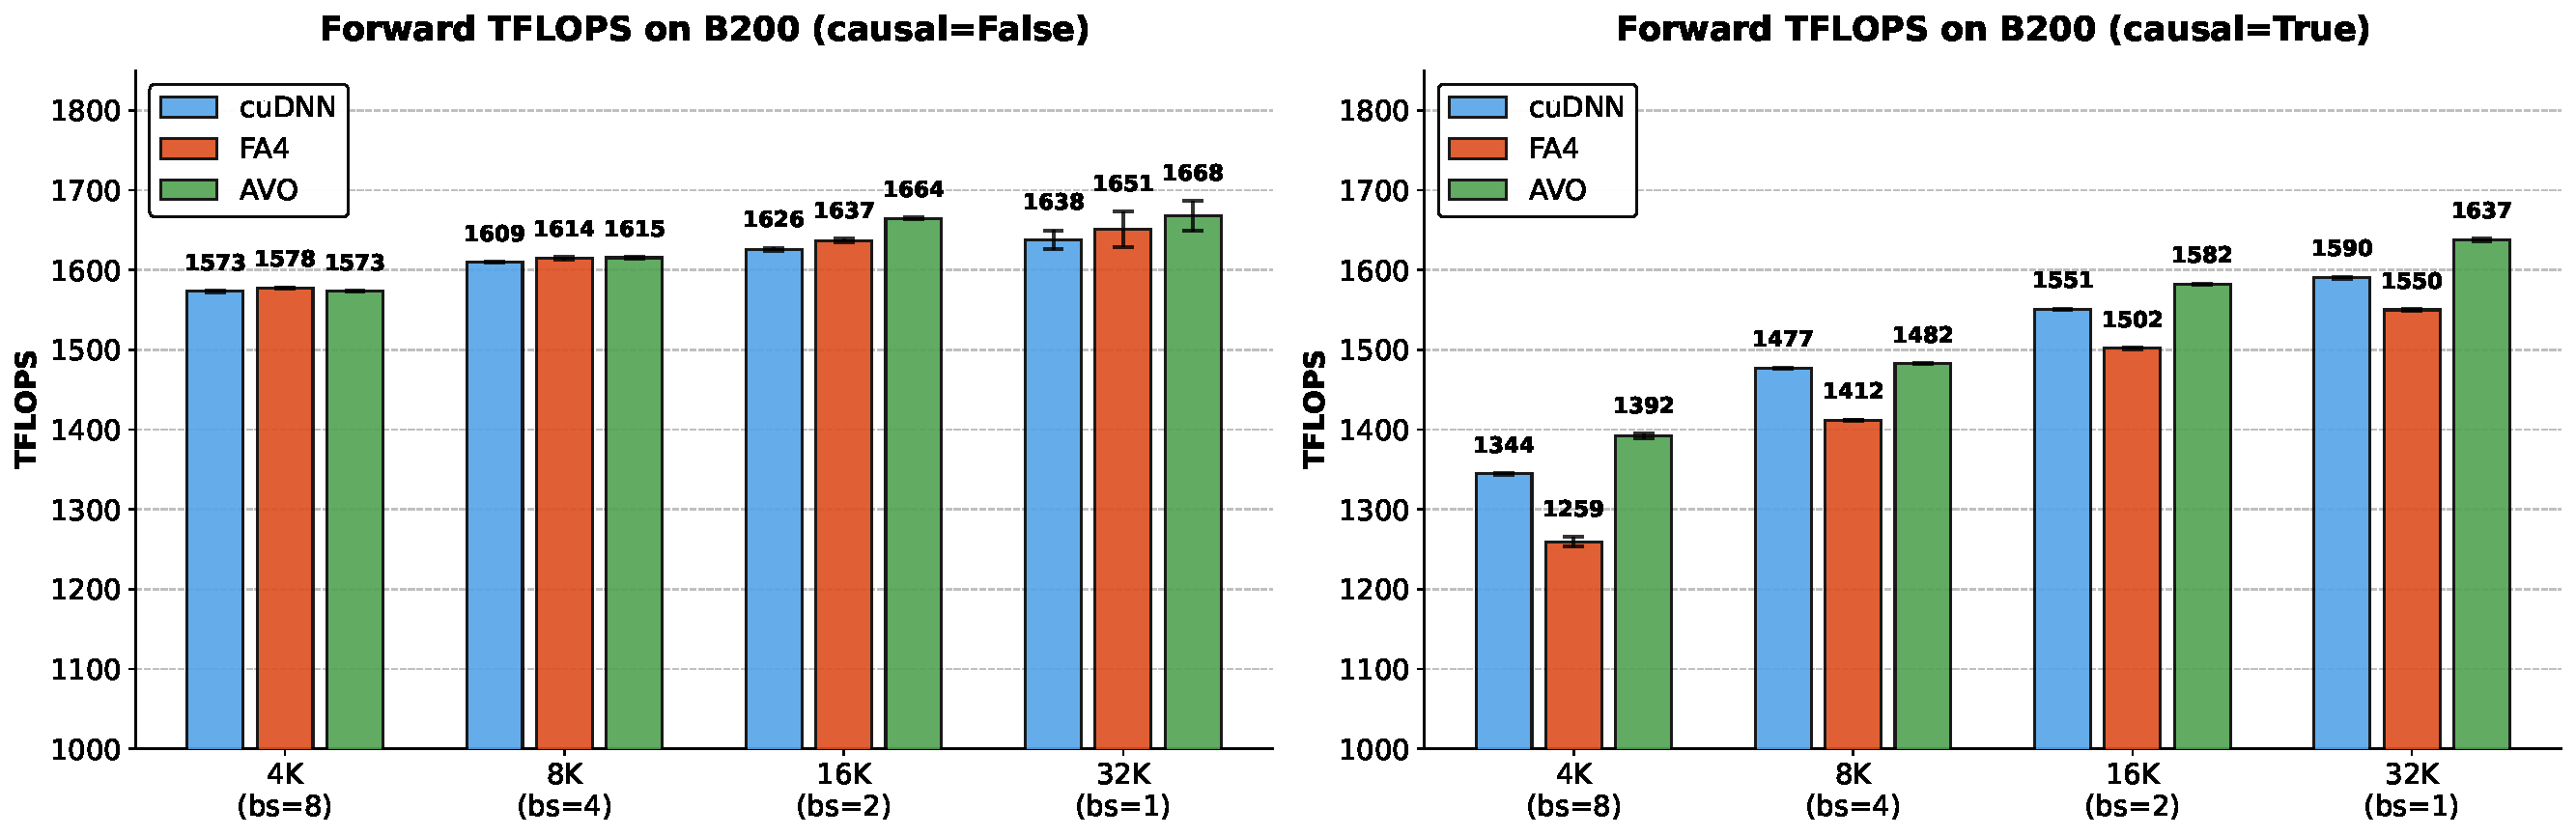
\includegraphics[width=\textwidth]{figures/mha_performance.pdf}
  \caption{Multi-head attention forward-pass prefilling throughput (TFLOPS) on NVIDIA B200 with head dimension 128, 16 heads, and BF16 precision. Batch size and sequence length are varied with a fixed total of 32k tokens.}
  \label{fig:mha_results}
\end{figure}

\subsection{Grouped-Query Attention}
\label{sec:results_gqa}

To evaluate whether agent-discovered optimizations transfer beyond the benchmark settings used in evolution, we prompted the AVO agent to adapt the evolved MHA kernel to support GQA.
The agent completed this adaptation autonomously in approximately 30 minutes, producing a GQA-capable kernel without any human guidance on the required changes.

Figure~\ref{fig:gqa_results} presents the results across two GQA configurations.
AVO outperforms both baselines across all configurations.
On causal GQA, AVO achieves up to $+7.0\%$ over cuDNN and $+9.3\%$ over FA4.
On non-causal GQA, gains reach up to $+6.0\%$ over cuDNN and $+4.5\%$ over FA4.
The strong GQA performance demonstrates that the optimizations discovered by the agent during MHA evolution are not specific to the MHA configurations used during evolution, but generalize to the distinct compute and memory access patterns of GQA.

\begin{figure}[t]
  \centering
  
   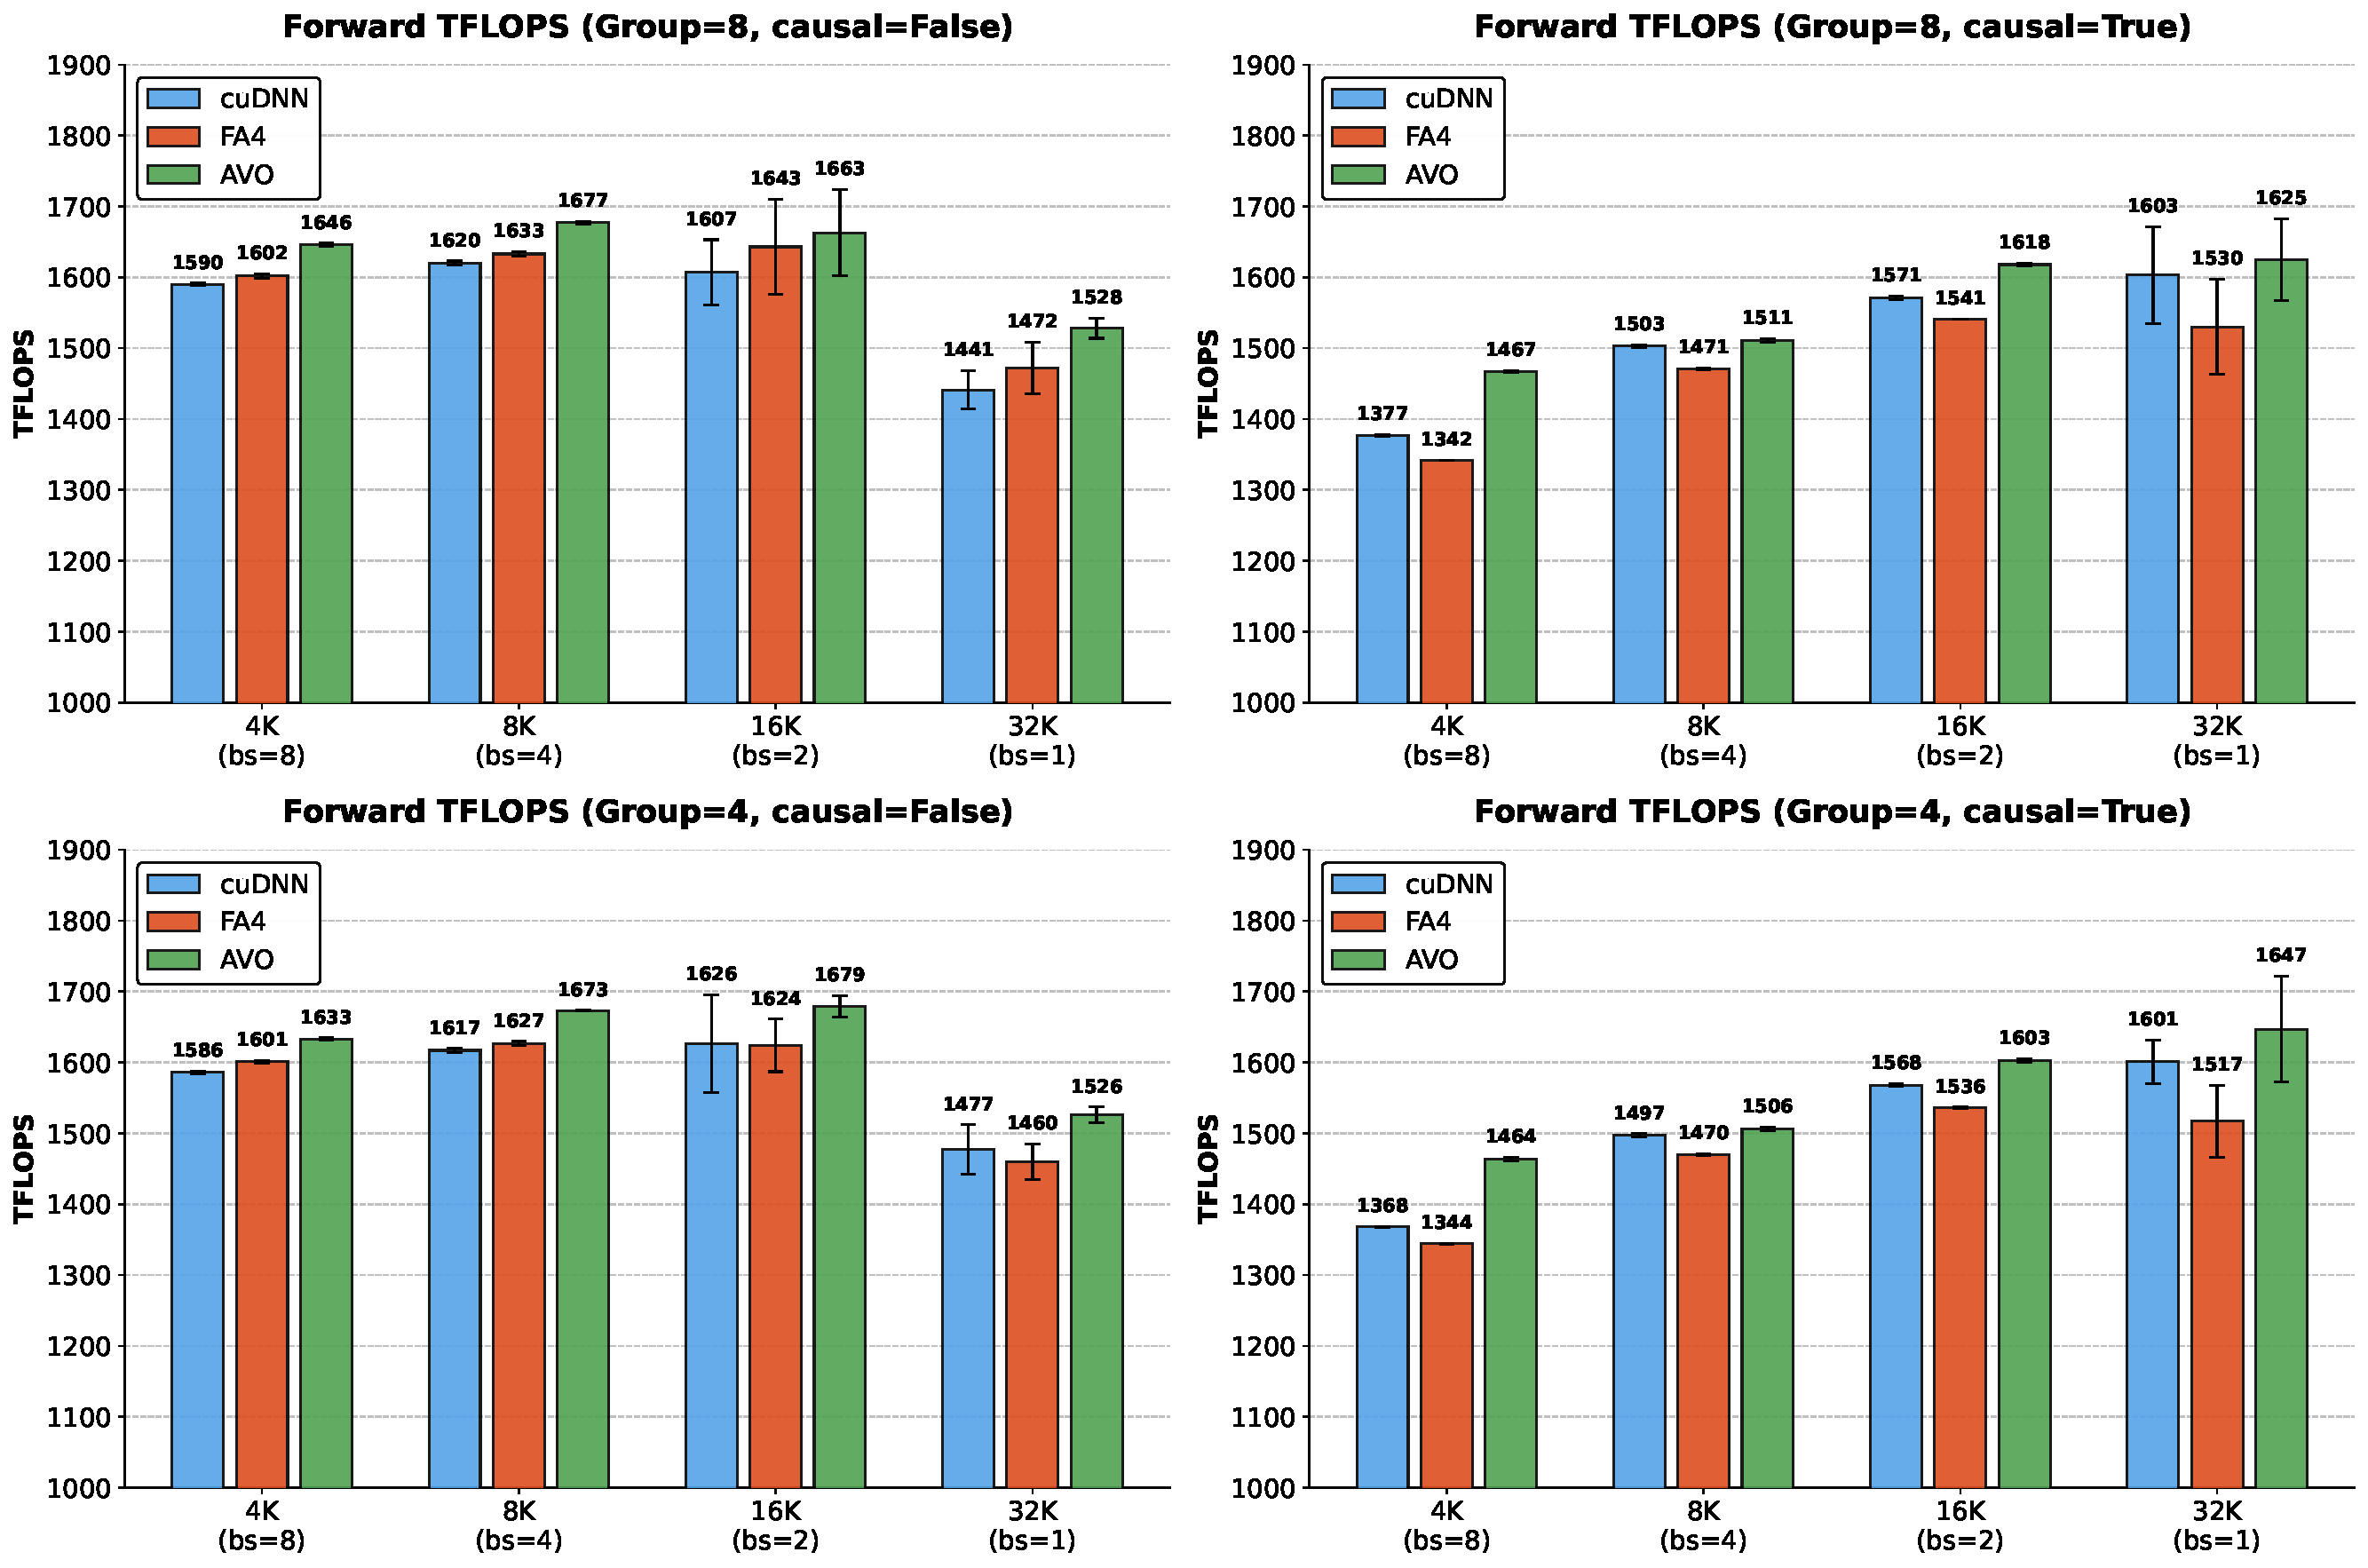
\includegraphics[width=\textwidth]{figures/gqa_performance.pdf}
  \caption{Grouped-query attention forward-pass prefilling throughput (TFLOPS) on NVIDIA B200 with 32 query heads, head dimension 128 and BF16 precision. Results are shown for two GQA configurations (group sizes 8 and 4) under both causal and non-causal masking. The GQA kernel was produced by prompting the AVO agent to adapt the evolved MHA kernel, requiring approximately 30 minutes of autonomous effort.}
  \label{fig:gqa_results}
\end{figure}

\subsection{Evolution Trajectory}
\label{sec:results_trajectory}

In Figure~\ref{fig:evolution_causal_trajectory} and Figure~\ref{fig:evolution_noncausal_trajectory}, we show the evolution trajectory of AVO across the 40 committed kernel versions produced during the 7-day evolution.
Note that these trajectories visualize the committed sequence, rather than the full internal search tree explored between the commits.
We observed the following patterns:

\paragraph{Scale of exploration.}
The 40 committed versions shown in the trajectory represent only the successful outcomes of a much larger search.
Over the 7-day evolution, the agent explored over 500 candidate optimization directions internally, including attempts that failed correctness checks, regressed throughput, or were abandoned after profiling.
This volume of systematic exploration, each direction requiring reading documentation, implementing changes, compiling, testing, and profiling, far exceeds what a human engineer could accomplish in the same timeframe.

\paragraph{Discrete jumps rather than gradual improvement.}
Throughput improves in distinct steps separated by plateaus where successive versions refine implementation details without measurably changing performance.
The five largest gains correspond to architectural inflection points: the introduction of QK-PV interleaving with bitmask causal masking (version 8), a restructured single-pass softmax computation (version 13), the branchless accumulator rescaling with a lighter memory fence for unmasked iterations (version 20), the correction/MMA pipeline overlap (version 30), and register rebalancing across warp groups (version 33). We discuss some of the representative optimizations in Section~\ref{sec:analysis}.
The remaining versions contribute individually smaller but collectively substantial micro-architectural refinements.

\paragraph{Diminishing returns.}
The earlier versions (v1 through v20) deliver the largest absolute gains per version, closing the gap between a naive implementation and the well-optimized baselines.
The later versions (v21 through v40) yield smaller but compounding improvements through cycle-level scheduling and refined resource allocation.
This pattern is consistent with the general observation that early kernel development captures coarse-grained gains while late-stage optimization squeezes out remaining headroom through increasingly fine-grained tuning.

\begin{figure}[t]
  \centering
  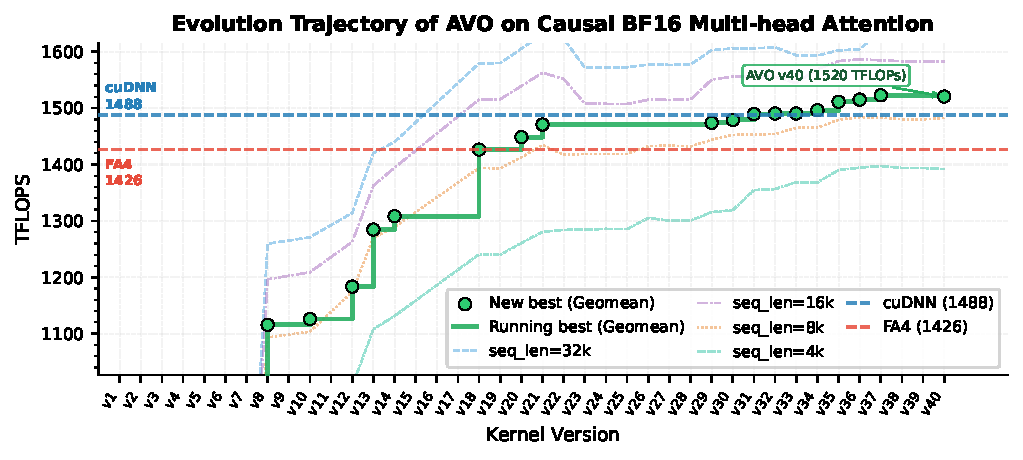
\includegraphics[width=\textwidth]{figures/avo_mha_causal_neurips.pdf}
  \caption{Evolution trajectory of AVO across 40 kernel versions over 7 days on \textbf{causal} MHA. The solid green line tracks the running-best geometric mean throughput across all configurations; green circles mark versions that set a new best. Dashed colored lines show per-configuration throughput (seq\_len = 4k, 8k, 16k, 32k). Horizontal dashed lines indicate the geometric mean throughput of cuDNN and FA4.}
  \label{fig:evolution_causal_trajectory}
\end{figure}

\begin{figure}[t]
  \centering
  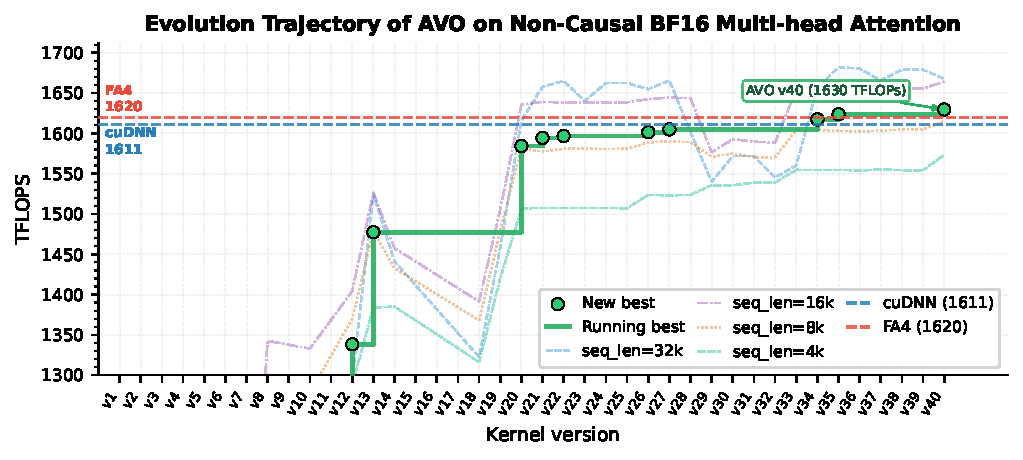
\includegraphics[width=\textwidth]{figures/avo_mha_noncausal_neurips.pdf}
  \caption{Evolution trajectory of AVO across 40 kernel versions over 7 days on \textbf{non-causal} MHA. The solid green line tracks the running-best geometric mean throughput across all configurations; green circles mark versions that set a new best. Dashed colored lines show per-configuration throughput (seq\_len = 4k, 8k, 16k, 32k). Horizontal dashed lines indicate the geometric mean throughput of cuDNN and FA4.}
  \label{fig:evolution_noncausal_trajectory}
\end{figure}
